\documentclass[11pt]{article}
\usepackage[margin=1in]{geometry}
\usepackage{amsmath,amssymb,amsthm,mathrsfs,mathtools}
\usepackage{xcolor}
\usepackage{hyperref}
\usepackage{orcidlink}
\usepackage{tikz}
\hypersetup{colorlinks=true,linkcolor=blue!60!black,citecolor=blue!60!black,urlcolor=blue!60!black}

\newcommand{\Srel}{S^{\mathrm{rel}}}
\newcommand{\Nariai}{Nariai}

\title{\textbf{The Linear-Response Postulate Is a Theorem:}\\ Jackiw--Teitelboim Dynamics and the Area Law on the \Nariai{} Horizon}
\author{Brent S. Hartshorn \orcidlink{0009-0004-2853-655X} (\url{brenthartshorn@proton.me})}

\begin{document}
\maketitle

\begin{abstract}
Dorau and Much have shown that the semiclassical Einstein equations follow from Tomita--Takesaki modular theory on a bifurcate Killing horizon, given the identification $\Srel = \delta A/4$ of the Araki--Uhlmann relative entropy of a coherent excitation with one quarter of the horizon area variation~\cite{DorauMuch}. One ingredient of that derivation is a postulate: a linear-response model for how the area answers the flux. We show that on the \Nariai{} spacetime $dS_2 \times S^2$ --- the degenerate limit of Schwarzschild--de~Sitter in which the two horizons merge --- this postulate is a theorem. The $s$-wave backreaction of the throat is exactly linearized de~Sitter Jackiw--Teitelboim gravity, its dilaton equation admits the response model as the unique zero-mode-free solution, and the coupling $8\pi$ is fixed by the dimensional reduction rather than imported from Bekenstein--Hawking. The relative entropy of coherent excitations is computed on this background by the method of Kurpicz, Pinamonti and Verch and of Dorau and Much; what is new is the arena, whose degenerate surface gravities admit a single global KMS state and whose Killing normalization is fixed by the geometry, and the theorem. Positivity of the relative entropy then selects a branch of the \Nariai{} instability: coherent matter flux drives the pierced horizon cut up and cannot realize anti-evaporation.
\end{abstract}

\section{Introduction}
\label{sec:intro}

Jacobson's 1995 observation that the Einstein equations can be recovered from the Clausius relation $\delta Q = T\,\delta S$ applied to local Rindler horizons recast gravity as thermodynamics \cite{Jacobson}: an equation of state rather than a fundamental force law. The argument, however, borrowed its entropy from black-hole thermodynamics wholesale, leaving unspecified both the statistical system to which that entropy belongs and the quantum theory in which the heat flux $\delta Q$ is defined. Dorau and Much have recently closed the second gap \cite{DorauMuch}: working entirely within algebraic quantum field theory, they showed that the Araki--Uhlmann relative entropy between a quasifree vacuum state $\omega_0$ and its coherent excitation $\omega_\phi$, evaluated on the horizon algebra of a bifurcate Killing horizon, is
\begin{equation}
\Srel(\omega_0 \,\|\, \omega_\phi)
= -2\pi \int_{\mathcal{H}^{\mathcal{R}}} U \,\langle{:}T_{ab}{:}\rangle_{\omega_\phi}\, \xi^a \xi^b \, dU\, d\mathrm{vol}_{\mathcal{S}},
\label{eq:DM-pivot}
\end{equation}
i.e.\ precisely the boost-energy flux that plays the role of $\delta Q$ in Jacobson's argument \cite{Jacobson}. The heat is no longer thermodynamic bookkeeping; it is a theorem of modular theory. Assuming the Bekenstein--Hawking normalization $\Srel = \delta A/4$ then fixes the coupling of the resulting field equations to $8\pi$, and the semiclassical Einstein equations follow.

This theorem-driven route contrasts with the parallel ``gravity from entropy'' proposal of Bianconi \cite{Bianconi2025,Bianconi2026}, in which the gravitational action is \emph{defined} as a quantum relative entropy between the spacetime metric and a matter-induced metric, and modified Einstein equations follow by variation --- at the price of truncations (a reduced Dirac--K\"ahler field content, an auxiliary-field reformulation) whose consistency with the general theory is not demonstrated. The route pursued here is complementary: no new action and no truncation, but a chain of theorems --- modular theory on an exact solution --- in which every quantity is finite and every step is either derived or explicitly flagged as a postulate. The two programs converge on the question both must ultimately answer: what the entropy that sources gravity is an entropy \emph{of}.

Dorau and Much state their result as a biconditional: assuming $\Srel = \delta A/4$ one recovers the semiclassical Einstein equations, and conversely \cite{DorauMuch}. What the derivation does not supply, and does not claim to supply, is a reason for that normalization. The relative entropy itself is unambiguous --- it is the distinguishability of a coherent excitation from the vacuum, and Bianconi's construction is likewise explicit about its two arguments, the spacetime metric and the matter-induced metric \cite{Bianconi2025} --- but the factor $1/4$ imports a statement about gravitational microstates from black-hole thermodynamics, and with it a linear-response model, first order in the metric perturbation, for how the area answers the flux. That model is a postulate of the derivation.

It is this postulate, and not the finiteness of any area, that the present paper removes. We claim no advantage from the compactness of the bifurcation surface as regards the entropy itself: the Araki--Uhlmann entropy of a coherent excitation equals an area \emph{variation}, which is well defined when the cross-section is non-compact, as the Rindler case and the general analysis of Ref.~\cite{DAngelo} both show. Nothing below turns on replacing $\delta A$ by $A$.

What the \Nariai{} geometry $dS_2 \times S^2$ --- the degenerate limit of the Schwarzschild--de~Sitter family in which the black-hole and cosmological horizons merge at the common radius $r = 1/\sqrt{\Lambda}$ \cite{Nariai} --- does supply is three things the Rindler wedge and the generic Schwarzschild--de~Sitter member do not. The surface gravities of the two horizons degenerate, so a single Killing flow governs the whole horizon and a global KMS state exists, where at generic mass the two horizons carry different temperatures and no global equilibrium state is available. The normalization of that Killing field is fixed by the geometry through the Bousso--Hawking prescription \cite{BoussoHawking} rather than by a choice of boost parameter, so $\delta Q$ and $\Srel$ are separately unambiguous rather than only their ratio. And the background sits at an unstable equilibrium whose two branches the positivity of relative entropy can distinguish; the instability also threatens the rigid Killing horizon on which the modular machinery is erected, and Section~\ref{sec:timescales} meets this with a quantitative separation of timescales, with the horizon entropy itself as hierarchy parameter.

The consequence of the first two is the result of this paper: on this background the $s$-wave backreaction of the throat is exactly linearized de~Sitter Jackiw--Teitelboim gravity (Section~\ref{sec:JT}), its dilaton equation admits the linear-response model as its unique zero-mode-free solution, and the coupling $8\pi$ is fixed by the dimensional reduction. The postulate of \cite{DorauMuch} becomes a theorem, and $\delta A = 4\,\Srel$ is derived rather than assumed.

\paragraph{What is taken from the literature, and what is new.} To keep the two apart: the scaling-limit two-point function and the modular structure on a bifurcate Killing horizon are due to Kay and Wald \cite{KayWald} and to Summers and Verch \cite{SummersVerch}; the formula for the relative entropy of a coherent excitation, and its identification with the boost-energy flux, are due to Kurpicz, Pinamonti and Verch \cite{KPV} and to Dorau and Much \cite{DorauMuch}, and Sections~\ref{sec:algebra}--\ref{sec:entropy} apply their results to \Nariai{} without modification; the dimensional reduction of the throat to de~Sitter JT gravity is standard \cite{MertensTuriaci}. New here are the timescale separation of Section~\ref{sec:timescales}, the closed-form $s$-wave family of Section~\ref{sec:example} with its exact Clausius relation, the theorem of Section~\ref{sec:JT} that the response model and its coupling follow from the JT dilaton equation, and the branch-selection argument of Section~\ref{sec:instability}.

The Dorau--Much quantity \eqref{eq:DM-pivot} is not a von Neumann entropy of a hidden substrate; it is a \emph{relative} entropy, the information-theoretic distinguishability of the realized state $\omega_\phi$ from the counterfactual vacuum $\omega_0$. It measures, in the only sense the algebraic theory makes available, how
much the world that happened differs from the world that did not.


% ====================================================================
\section{The \Nariai{} Geometry and its Bifurcate Killing Horizon}
\label{sec:geometry}

Throughout we use units $G = \hbar = c = 1$, so that areas, entropies and energies are measured in Planck units and the Einstein coupling appears as $8\pi$.

\subsection{The Schwarzschild--de Sitter family and its degenerate limit}

The Schwarzschild--de Sitter (SdS) family in four dimensions,
\begin{equation}
ds^2 = -f(r)\,dt^2 + \frac{dr^2}{f(r)} + r^2\, d\Omega^2,
\qquad
f(r) = 1 - \frac{2M}{r} - \frac{\Lambda r^2}{3},
\label{eq:SdS}
\end{equation}
possesses, for $0 < 9\Lambda M^2 < 1$, two positive roots of $f$: the black-hole horizon $r_b$ and the cosmological horizon $r_c > r_b$. Their surface gravities,
\begin{equation}
\kappa_{b,c} = \tfrac{1}{2}\,|f'(r_{b,c})|,
\end{equation}
are unequal for any nondegenerate member of the family. This inequality is why generic SdS is a poor arena for the algebraic construction of Ref.~\cite{DorauMuch}: the two horizons define inequivalent notions of thermal equilibrium, no globally regular Killing-invariant Hadamard state exists on the full extension (the obstruction identified by Kay and Wald~\cite{KayWald}), and any horizon-by-horizon treatment inherits an ambiguity in the reference state --- an ambiguity that the common remedy of partitioning SdS by timelike boundaries \cite{Rusalev} makes explicit rather than removes.

The degenerate limit removes the obstruction. As $9\Lambda M^2 \to 1$ the two roots merge at
\begin{equation}
r_b, r_c \;\to\; r_\star = \frac{1}{\sqrt{\Lambda}} = 3M,
\end{equation}
and the region between the horizons acquires a finite invariant description. Following the Ginsparg--Perry procedure~\cite{GinspargPerry}, set
\begin{equation}
9\Lambda M^2 = 1 - 3\varepsilon^2, \qquad 0 \le \varepsilon \ll 1,
\end{equation}
and introduce coordinates $(\psi, \chi)$ adapted to the near-degenerate throat,
\begin{equation}
t = \frac{\psi}{\varepsilon\sqrt{\Lambda}},
\qquad
r = \frac{1}{\sqrt{\Lambda}}\left(1 - \varepsilon\cos\chi \right) + \mathcal{O}(\varepsilon^2).
\end{equation}
In the limit $\varepsilon \to 0$ the metric \eqref{eq:SdS} becomes the \Nariai{} spacetime~\cite{Nariai}
\begin{equation}
ds^2 = \frac{1}{\Lambda}\left(-\sin^2\!\chi \, d\psi^2 + d\chi^2\right) + \frac{1}{\Lambda}\, d\Omega^2 ,
\label{eq:nariai-global}
\end{equation}
the direct product $dS_2 \times S^2$ of a two-dimensional de~Sitter factor and a round two-sphere, both of curvature radius $1/\sqrt{\Lambda}$. Unlike the near-horizon limits of asymptotically flat extremal black holes, \eqref{eq:nariai-global} is an exact solution of the Einstein equations with cosmological constant $\Lambda$, and it is the \emph{unique} member of the SdS family admitting a global bifurcate Killing horizon with a single surface gravity.


\begin{figure}[t]
\centering
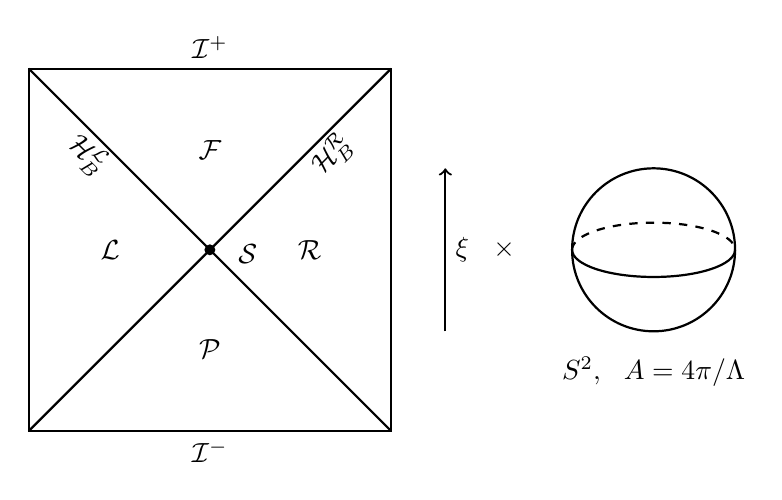
\begin{tikzpicture}[scale=1.15]
  % the dS_2 factor: a Penrose square with the bifurcate horizon
  \draw[thick] (-2,-2) rectangle (2,2);
  \draw[thick] (-2,-2) -- (2,2);
  \draw[thick] (-2,2) -- (2,-2);
  \node at (0,0) [circle,fill,inner sep=1.4pt] {};
  \node at (0.42,-0.05) {$\mathcal{S}$};
  \node at (1.1,0) {$\mathcal{R}$};
  \node at (-1.1,0) {$\mathcal{L}$};
  \node at (0,1.1) {$\mathcal{F}$};
  \node at (0,-1.1) {$\mathcal{P}$};
  \node[above] at (0,2) {$\mathcal{I}^+$};
  \node[below] at (0,-2) {$\mathcal{I}^-$};
  \node[rotate=45] at (1.35,1.05) {$\mathcal{H}^{\mathcal{R}}_B$};
  \node[rotate=-45] at (-1.35,1.05) {$\mathcal{H}^{\mathcal{L}}_B$};
  \draw[->,thick] (2.6,-0.9) -- (2.6,0.9) node[midway,right] {$\xi$};
  % the transverse sphere
  \draw[thick] (4.9,0) circle (0.9);
  \draw[thick] (4.0,0) arc (180:360:0.9 and 0.3);
  \draw[thick,dashed] (4.0,0) arc (180:0:0.9 and 0.3);
  \node at (4.9,-1.35) {$S^2,\ \ A = 4\pi/\Lambda$};
  \node at (3.25,0) {$\times$};
\end{tikzpicture}
\caption{The \Nariai{} geometry $dS_2 \times S^2$. Left: the conformal diagram of the $dS_2$ factor. The two null lines are the bifurcate Killing horizon, meeting at the bifurcation surface $\mathcal{S}$; $\mathcal{R}$ and $\mathcal{L}$ are the two static patches, in which the Killing field $\xi$ is timelike, and $\mathcal{F}$, $\mathcal{P}$ their future and past. The horizon algebra of Section~\ref{sec:algebra} lives on the future branch $\mathcal{H}^{\mathcal{R}}_B$ of the right wedge. Right: every point of the diagram is a round two-sphere of radius $1/\sqrt{\Lambda}$; the bifurcation surface is compact, with area $4\pi/\Lambda$. In generic Schwarzschild--de~Sitter the two null lines carry different surface gravities; in the degenerate limit they are equal, which is what makes a single Killing flow and a global KMS state available.}
\label{fig:nariai}
\end{figure}

\subsection{Static patch, horizon structure, and the normalization of the Killing field}
The geometry is drawn in Figure~\ref{fig:nariai}. 
Substituting $\rho = \Lambda^{-1/2}\cos\chi$ and $\tau = \Lambda^{-1/2}\psi$ brings the $dS_2$ factor to static form,
\begin{equation}
ds^2 = -\big(1-\Lambda\rho^2\big)\,d\tau^2 + \frac{d\rho^2}{1-\Lambda\rho^2} + \frac{1}{\Lambda}\,d\Omega^2 ,
\label{eq:nariai-static}
\end{equation}
with Killing field $\xi = \partial_\tau$ and Killing horizons at $\rho = \pm \Lambda^{-1/2}$. The surface gravity of $\xi$ is
\begin{equation}
\kappa = \sqrt{\Lambda}\,,
\qquad
T = \frac{\kappa}{2\pi} = \frac{\sqrt{\Lambda}}{2\pi}\,,
\label{eq:temperature}
\end{equation}
which is the Bousso--Hawking temperature of the degenerate solution~\cite{BoussoHawking}. Two remarks on normalization are essential, because this is the hinge on which the modular theory of Section~\ref{sec:algebra} turns. First, the limit must be taken in the rescaled time $\psi$, not in the SdS time $t$: the surface gravities $\kappa_{b,c}$ of the parent family both vanish as $\varepsilon \to 0$, and a construction anchored to $\partial_t$ would see zero temperature. The rescaling $t = \psi/(\varepsilon\sqrt{\Lambda})$ is the Bousso--Hawking prescription of normalizing the generator with respect to the inertial observer suspended between the horizons. Second --- and this is where \Nariai{} improves on the Rindler wedge --- the normalization is \emph{not} ambiguous. The Rindler boost generator admits arbitrary rescaling, correspondingly rescaling the Unruh temperature, a freedom Ref.~\cite{DorauMuch} notes as an intrinsic limitation of the local construction. On \Nariai{} the geometry itself supplies the scale: the Killing field in \eqref{eq:nariai-static} is fixed (up to sign) by unit normalization on the central geodesic $\rho = 0$, and the temperature \eqref{eq:temperature} is an invariant of the solution.

With $\rho_*$ the tortoise coordinate of \eqref{eq:nariai-static} and $u,v = \tau \mp \rho_*$, the affine (Kruskal-type) coordinates
\begin{equation}
U = -\frac{1}{\kappa}\,e^{-\kappa u},
\qquad
V = +\frac{1}{\kappa}\,e^{+\kappa v},
\end{equation}
extend the static patch to the full square Penrose diagram of $dS_2$, every point of which carries the sphere $S^2_{1/\sqrt{\Lambda}}$. The global null hypersurfaces $\mathcal{H}_B = \{V = 0\}$ and $\mathcal{H}_A = \{U = 0\}$, generated by the flow of $\xi$, intersect on the bifurcation surface
\begin{equation}
\mathcal{S} = S^2_{1/\sqrt{\Lambda}},
\qquad
A(\mathcal{S}) = \frac{4\pi}{\Lambda}\,,
\label{eq:area}
\end{equation}
a \emph{compact} two-sphere. The pair $(\mathcal{H}_A, \mathcal{H}_B)$ is a bifurcate Killing horizon in the exact sense of Kay and Wald~\cite{KayWald}, realized globally rather than as a local approximation, with cross-sectional volume element $d\mathrm{vol}_{\mathcal{S}} = \Lambda^{-1}\sin\theta\, d\theta\, d\varphi$ integrating to the finite total \eqref{eq:area}. Every transverse integral in Sections~\ref{sec:algebra} and~\ref{sec:entropy} is therefore finite from the outset, and the associated horizon entropy
\begin{equation}
S_{\mathrm{N}} = \frac{A(\mathcal{S})}{4} = \frac{\pi}{\Lambda}
\label{eq:Smax}
\end{equation}
is not only finite but extremal: it saturates the maximal horizon entropy attainable within the SdS family at fixed $\Lambda$. The \Nariai{} horizon is, in this precise sense, the largest ledger de~Sitter space affords.

\subsection{Global hyperbolicity and the Euclidean section}

Two further structural facts prepare the ground. First, $dS_2 \times S^2$ is globally hyperbolic (a product of globally hyperbolic $dS_2$ with a compact Riemannian factor), so the algebraic quantization of a Klein--Gordon field proceeds without the causal subtleties of generic SdS. Second, the Euclidean section obtained by $\psi \to -i\psi_E$ is the round product $S^2 \times S^2$, compact and everywhere regular, with thermal periodicity $\psi_E \sim \psi_E + 2\pi$ built into the geometry. There is consequently a distinguished Hartle--Hawking-type state $\omega_0$: obtained by analytic continuation from the regular Euclidean section, invariant under the Killing flow, Hadamard, and KMS at the temperature \eqref{eq:temperature}. For nondegenerate SdS no such globally regular equilibrium state exists --- the two unequal temperatures forbid it --- so the degeneracy of \Nariai{} is not a curiosity we tolerate but the very feature that makes a preferred global vacuum available. It is this $\omega_0$ that plays the role of the reference state: the ``unrealized'' side of the relative entropy.

\subsection{Vacuum polarization, the Ginsparg--Perry instability, and KMS}
\label{sec:timescales}

Tomita--Takesaki theory itself requires no geometry: a von Neumann algebra with a cyclic separating vector suffices. What requires geometry is the \emph{identification} of the modular flow with the Killing flow --- the Bisognano--Wichmann property and its curved-space form for bifurcate Killing horizons \cite{Sewell,KayWald} --- and it is that identification, on which the modular Hamiltonian of Section~\ref{sec:modularH} and hence the Araki--Uhlmann entropy rest, that presupposes a fixed bifurcate Killing horizon carrying an invariant KMS state $\omega_0$. But the \Nariai{} background is not inert: it is the unstable saddle governing the semiclassical decay of de~Sitter space \cite{GinspargPerry}, and one-loop vacuum polarization drives the degenerate geometry off the extremal point along the (anti-)evaporation branches \cite{BoussoHawking}. If the background is deformed by the very fields whose modular structure we exploit, in what sense is a \emph{static} modular Hamiltonian available? Treating the instability as a predictive bonus (Section~\ref{sec:instability}) while silently assuming a rigid background elsewhere would be inconsistent. The resolution is a separation of timescales, made quantitative on \Nariai{} because the hierarchy parameter turns out to be the horizon entropy itself.

Three timescales are in play. The first is the modular (thermal) time: one period of Euclidean periodicity, or equivalently the light-crossing time of the throat,
\begin{equation}
t_{\mathrm{mod}} \;=\; \beta \;=\; \frac{2\pi}{\kappa} \;=\; \frac{2\pi}{\sqrt{\Lambda}}\,.
\label{eq:t-mod}
\end{equation}
This is the timescale on which the modular flow \eqref{eq:dilations} acts, on which the KMS condition is formulated, and on which the horizon data of a localized excitation live. The second is the classical evolution timescale of the branch parameter $\varepsilon$ --- and here the first structural point enters: \emph{there is none}. Within classical general relativity, $\varepsilon$ labels a one-parameter family of exactly static solutions \eqref{eq:SdS}; the degenerate point sits on a flat direction, not a classical instability. The \Nariai{} instability is an $\mathcal{O}(\hbar)$ effect from the start, sourced entirely by the renormalized stress tensor fed back through the semiclassical Einstein equations. The third timescale is therefore the backreaction time. Dimensionally, a Hadamard state on a background of curvature radius $r_\star = 1/\sqrt{\Lambda}$ has $\langle T_{ab}\rangle_{\mathrm{ren}} \sim \hbar\,\Lambda^2$ per field species; inserted into $G_{ab} + \Lambda g_{ab} = 8\pi\, \langle T_{ab}\rangle_{\mathrm{ren}}$, it drives the dimensionless perturbation at a rate
\begin{equation}
\Gamma \;\sim\; \underbrace{\kappa}_{\substack{\text{modular}\\ \text{frequency}}} \cdot \underbrace{\big(G\hbar\,\Lambda\big)}_{\substack{\text{semiclassical}\\ \text{parameter } \ell_P^2/r_\star^2}}
\;=\; \frac{\pi\,\kappa}{S_{\mathrm{N}}}\,,
\qquad
S_{\mathrm{N}} = \frac{\pi}{G\hbar\,\Lambda}\,,
\label{eq:Gamma}
\end{equation}
which is the parametric content of the Bousso--Hawking analysis \cite{BoussoHawking}: the perturbation $\varepsilon$ grows (or decays) on a timescale longer than the modular time by a factor of order the horizon entropy,
\begin{equation}
\frac{t_{\mathrm{inst}}}{t_{\mathrm{mod}}} \;\sim\; \frac{S_{\mathrm{N}}}{\pi} \;\gg\; 1\,.
\label{eq:hierarchy}
\end{equation}
The nucleation channel is suppressed more strongly still: the Ginsparg--Perry decay of de~Sitter proceeds through the $S^2 \times S^2$ instanton --- the Euclidean section of Section~\ref{sec:geometry} itself --- at a rate $\propto e^{-(I_{\mathrm{N}} - I_{dS})} = e^{-S_{\mathrm{N}}}$ \cite{GinspargPerry}. For any macroscopic value of the cosmological constant $S_{\mathrm{N}}$ is enormous (of order $10^{122}$ for the observed $\Lambda$), and the hierarchy \eqref{eq:hierarchy} is not merely large but the largest in physics.

The consequences for the modular construction are:

\emph{(a) Order counting.} Sections~\ref{sec:algebra} and \ref{sec:entropy} are exact statements about the fixed background --- the zeroth-order term in an expansion in $G\hbar\Lambda = \pi/S_{\mathrm{N}}$; the instability and the area response \eqref{eq:perturbation} are first-order in the same parameter. Using zeroth-order modular data inside a first-order response equation is the standard, and only consistent, semiclassical truncation --- the same one implicit in Refs.~\cite{Jacobson,DorauMuch}; corrections from the drifting background are $\mathcal{O}(1/S_{\mathrm{N}})$, the order of loop corrections already discarded in writing semiclassical gravity at all.

\emph{(b) Kinematic rigidity.} The entropy formula depends on the background through exactly two structures: the Kay--Wald scaling-limit kernel \eqref{eq:scaling-limit}, universal and hence blind to a slow drift; and the transverse measure $d\mathrm{vol}_{\mathcal{S}}$, which drifts fractionally by $\mathcal{O}(\kappa\,\Delta u / S_{\mathrm{N}})$ over the boost-time support $\Delta u$ of an excitation.

\emph{(c) The quasi-equilibrium window.} For any excitation whose \emph{modular support} --- the extent $\Delta u$ of its profile in boost time, the parameter of the modular flow \eqref{eq:dilations} --- satisfies $\kappa\,\Delta u \ll S_{\mathrm{N}}$ --- satisfied with $\sim 120$ orders of magnitude to spare by anything localized --- the KMS state, the modular flow, and the relative entropy \eqref{eq:Srel-nariai} are valid up to relative corrections of order $1/S_{\mathrm{N}}$; the modular theory of this paper is the theory of that window, before accumulated backreaction ruptures the degenerate structure at $t \sim S_{\mathrm{N}}\,\beta$.

Two remarks. The hierarchy is not imposed but \emph{self-generated}: a single coherent excitation shifts the area fractionally by $\delta A/A = (\Lambda/\pi)\,\Srel$ in Planck units (Section~\ref{sec:entropy}) --- $\mathcal{O}(1/S_{\mathrm{N}})$ per nat --- so the rate at which the equilibrium description degrades is the rate at which the framework's own first-order output accumulates: the theory predicts the size of its domain of validity, Eq.~\eqref{eq:hierarchy}. Conversely, at times $\sim S_{\mathrm{N}}\beta$, or near the branch endpoints, no static modular Hamiltonian exists and the present framework makes no claim; what replaces it is the dynamical problem of backreaction under sign-indefinite flux, the open frontier noted in Section~\ref{sec:scope}.

\section{Horizon Algebra and Modular Structure on \Nariai{}}
\label{sec:algebra}

\subsection{Field content and dimensional reduction}

Let $\Phi$ be a real, minimally coupled Klein--Gordon field of mass $m$ on $dS_2 \times S^2$. The product structure separates the wave operator,
\begin{equation}
\square_g = \square_{dS_2} + \Lambda\, \Delta_{S^2},
\end{equation}
so expanding in spherical harmonics, $\Phi = \sum_{\ell m} \varphi_{\ell m}(\psi,\chi)\, Y_{\ell m}(\theta,\varphi)$, reduces the theory to an infinite tower of two-dimensional fields $\varphi_{\ell m}$ on $dS_2$ with effective masses
\begin{equation}
m_\ell^2 = \underbrace{m^2}_{\text{bare mass}} + \underbrace{\Lambda\,\ell(\ell+1)}_{\substack{\text{Kaluza--Klein mass}\\ \text{from the compact } S^2}}, \qquad \ell = 0, 1, 2, \dots
\label{eq:tower}
\end{equation}
The scaling limit below is insensitive to the tower, but \eqref{eq:tower} does two jobs. It exhibits the compactness of $\mathcal{S}$ as a physical regulator --- the transverse degrees of freedom are a discrete tower rather than a continuum, which is ultimately why the entropy integrals of Section~\ref{sec:entropy} converge without subtraction --- and it explains \emph{why} the $s$-wave sector $\ell = 0$ dominates near-horizon physics. On the $dS_2$ factor, of Hubble rate $\sqrt{\Lambda}$, every $\ell \ge 1$ member of \eqref{eq:tower} is a heavy, principal-series field, $m_\ell^2/\Lambda \ge 2 > \tfrac{1}{4}$, with $\nu_\ell = \sqrt{\ell(\ell+1) + m^2/\Lambda - \tfrac{1}{4}}$; its static-patch correlators decay rapidly and its thermal excitation is Boltzmann-suppressed as $e^{-\pi\nu_\ell} \sim e^{-\pi\ell}$. Each successive harmonic decouples exponentially from the near-horizon dynamics, so the restriction of the slow dynamics to the transversally homogeneous mode --- relied upon throughout Sections~\ref{sec:timescales} and~\ref{sec:instability} --- is enforced by the reduced mass spectrum itself: the compact sphere regulates both the entropy sums and the mode content of the instability.

\subsection{The scaling-limit two-point function on a compact horizon}

By the Kay--Wald analysis~\cite{KayWald}, the restriction of any Killing-flow-invariant Hadamard state to $\mathcal{H}_B$ possesses the universal scaling-limit two-point function; on \Nariai{} it takes exactly the form of Ref.~\cite{DorauMuch},
\begin{equation}
\Lambda_2(\phi, \psi)
= -\frac{1}{\pi} \int
\frac{\phi(U, s)\, \psi(U', s)}{(U - U' - i0^+)^2}\;
dU\, dU'\, d\mathrm{vol}_{\mathcal{S}},
\label{eq:scaling-limit}
\end{equation}
for $\phi, \psi \in C^\infty_c(\mathcal{H}_B)$, where now $s = (\theta,\varphi)$ ranges over the \emph{compact} bifurcation sphere and $d\mathrm{vol}_{\mathcal{S}} = \Lambda^{-1} \sin\theta\, d\theta\, d\varphi$. Three properties deserve emphasis.

\begin{enumerate}
\item \emph{Universality survives compactification.} The kernel in $U$ is the same conformal kernel as in the Rindler and Schwarzschild cases: the scaling limit forgets the mass tower \eqref{eq:tower} and the $dS_2$ curvature, retaining only the null-line conformal structure and the transverse measure. The horizon theory is effectively a chiral theory in $U$ fibered over $\mathcal{S}$ --- but the fiber integral is now finite.

\item \emph{The reference state is canonical.} On the Rindler horizon the state whose restriction yields \eqref{eq:scaling-limit} is the Minkowski vacuum; on \Nariai{} it is the Euclidean state $\omega_0$ of Section~\ref{sec:geometry}, distinguished by regularity on $S^2\times S^2$ and KMS at $\beta = 2\pi/\sqrt{\Lambda}$ with respect to the projected Killing flow.

\item \emph{The symplectic structure is finite.} Its finiteness is not a consequence of the compactness of $\mathcal{S}$ --- it holds equally for a non-compact cross-section --- but of the compact support of the test functions on which it is defined; what compactness of $\mathcal{S}$ gives is that the transverse decomposition is a discrete sum. The imaginary part of \eqref{eq:scaling-limit} equips $C^\infty_c(\mathcal{H}_B^{\mathcal{R}})$ with the symplectic form
\begin{equation}
\sigma(\phi,\psi)
= \int \big(\phi\,\partial_U \psi - \psi\,\partial_U \phi\big)\, dU\, d\mathrm{vol}_{\mathcal{S}},
\label{eq:symplectic}
\end{equation}
finite, by compactness of $\mathcal{S}$, even for data merely bounded in the transverse directions --- in particular for the homogeneous ($\ell = 0$) perturbations relevant to the instability, which on the Rindler horizon are not admissible test data. This enlargement of the admissible perturbation space is what gives Section~\ref{sec:instability} its content.

\end{enumerate}


\subsection{Weyl algebra, modular dilations, and the KMS structure}

The horizon von Neumann algebra now proceeds verbatim along Ref.~\cite{DorauMuch} and the modular analysis of Summers and Verch~\cite{SummersVerch}. Over $\big(C_c^\infty(\mathcal{H}_B^{\mathcal{R}}), \sigma\big)$ one builds the Weyl algebra $\mathscr{W}_{\mathcal{R}}$, generated by unitaries $W(\phi)$ satisfying
\begin{equation}
W(\phi)^\dagger = W(-\phi),
\qquad
W(\phi) W(\psi) = e^{-\frac{i}{2}\sigma(\phi,\psi)}\, W(\phi+\psi),
\end{equation}
represents it in the GNS representation $(\mathscr{H}_0, \pi_0, \Omega_0)$ of the quasifree state
\begin{equation}
\omega_0\big(W(\psi)\big) = e^{-\frac{1}{2}\Lambda_2(\psi,\psi)},
\end{equation}
and takes the double commutant $\mathscr{N}_{\mathcal{R}} = \pi_0(\mathscr{W}_{\mathcal{R}})''$. The vector $\Omega_0$ is cyclic and separating for $\mathscr{N}_{\mathcal{R}}$, and the associated Tomita--Takesaki modular group acts geometrically as affine dilations of the horizon generators,
\begin{equation}
\Delta_{\mathcal{R}}^{it} = \mathfrak{D}_{-2\pi t}:
\qquad
\phi(U, s) \;\longmapsto\; \phi\big(e^{-2\pi t}\, U,\; s\big),
\label{eq:dilations}
\end{equation}
leaving the compact transverse coordinate $s$ untouched; the orientation of the flow (contraction of $\mathcal{H}_B^{\mathcal{R}}$, where $U<0$, toward the bifurcation surface as $t \to +\infty$) is fixed by the KMS condition for $\omega_0$ and is the orientation that renders the relative entropy non-negative. This is the Bisognano--Wichmann property in its bifurcate-horizon generalization: it delivers, as a theorem rather than an input, the identification of the geometric Killing flow with the modular flow of $(\mathscr{N}_{\mathcal{R}}, \Omega_0)$ at the Bousso--Hawking temperature \eqref{eq:temperature}.

\subsection{The modular Hamiltonian in explicit form}
\label{sec:modularH}

For the computations of Section~\ref{sec:entropy} it is worth descending to explicit formulas. Differentiating \eqref{eq:dilations} at $t=0$, the generator $K = -\ln \Delta_{\mathcal{R}}$ acts on horizon data as $2\pi\, U \partial_U$, and its second-quantized form on the full horizon is the modular-weighted flux operator
\begin{equation}
K \;=\; -\ln \Delta_{\mathcal{R}}
\;=\; \underbrace{2\pi \int_{\mathcal{S}} d\mathrm{vol}_{\mathcal{S}} \int_{-\infty}^{0} (-U)\, {:}T_{UU}(U,s){:}\; dU}_{\displaystyle K_{\mathcal{R}}\;(\text{right-portion boost energy})}
\;-\;
\underbrace{2\pi \int_{\mathcal{S}} d\mathrm{vol}_{\mathcal{S}} \int_{0}^{\infty} U\, {:}T_{UU}(U,s){:}\; dU}_{\displaystyle K_{\mathcal{L}}\;(\text{left portion})}\,,
\label{eq:modularH}
\end{equation}
with $K_{\mathcal{R}}$ affiliated to $\mathscr{N}_{\mathcal{R}}$ and generating the dilations \eqref{eq:dilations} on $\mathcal{H}_B^{\mathcal{R}}$. Both integrals are individually finite in expectation on Hadamard excitations of $\omega_0$: the modular weight $|U|$ vanishes linearly at the bifurcation surface while the normal-ordered flux is integrable along the generators, and the transverse integral is bounded by the total area \eqref{eq:area}. On the Rindler horizon the same expression exists only as a formal density in the transverse plane; on \Nariai{} it is an honest (unbounded, self-adjoint) operator expression with finite state-dependent expectation values.

Equation \eqref{eq:modularH} is the null-coordinate face of the modular Hamiltonian. Its static face follows from the Bisognano--Wichmann identification: $K_{\mathcal{R}} = \beta\, H_\xi$ with $\beta = 2\pi/\sqrt{\Lambda}$, where $H_\xi$ is the Killing energy on a static slice $\Sigma_\tau$ of \eqref{eq:nariai-static}. With $\sqrt{h}\, d\rho\, d\Omega = (1-\Lambda\rho^2)^{-1/2}\, \Lambda^{-1} \sin\theta\, d\rho\, d\theta\, d\varphi$ and $n^a = (1-\Lambda\rho^2)^{-1/2}\, \delta^a_{\;\tau}$,
\begin{equation}
K_{\mathcal{R}} \;=\; \frac{2\pi}{\sqrt{\Lambda}}\; H_\xi\,,
\qquad
H_\xi
= \int_{\Sigma_\tau} T_{ab}\, \xi^a n^b\, d\Sigma
= \frac{1}{\Lambda} \int_{S^2} d\Omega \int_{-1/\sqrt{\Lambda}}^{\,1/\sqrt{\Lambda}}
\frac{{:}T_{\tau\tau}(\rho, s){:}}{1 - \Lambda \rho^2}\; d\rho\,,
\label{eq:KillingH}
\end{equation}
the energy flux integrated across the full throat, between the two poles of the degenerate horizon. The apparent divergence of the measure at $\rho \to \pm 1/\sqrt{\Lambda}$ is compensated for Hadamard states by $T_{\tau\tau} \propto (1-\Lambda\rho^2)$; and because the geometry fixes the normalization of $\xi$ (Section~\ref{sec:geometry}), the Killing energy \eqref{eq:KillingH} carries no rescaling ambiguity. The two faces \eqref{eq:modularH} and \eqref{eq:KillingH} are related on-shell by deforming $\Sigma_\tau$ to the horizon; the boost-Jacobian identity $(-U)\,(\partial_U\chi)^2\,dU = \kappa^{-1}(\partial_u\chi)^2\,du$, with $U = -\kappa^{-1}e^{-\kappa u}$ the boost time on the horizon, is precisely this deformation in coordinates. For wedge-local excitations --- coherent states here, squeezed states in \cite{SuppNariai} --- the general sum rule $\Srel(\omega_0\,\|\,\omega) = \Delta\langle K_{\mathcal{R}}\rangle - \Delta S$ with $\Delta S = 0$ reduces the Araki--Uhlmann relative entropy to the expectation-value shift of \eqref{eq:modularH},
\begin{equation}
\Srel(\omega_0\,\|\,\omega) \;=\; \langle K_{\mathcal{R}} \rangle_{\omega} - \langle K_{\mathcal{R}} \rangle_{\omega_0}\,,
\label{eq:Srel-K}
\end{equation}
which is the form in which the explicit computations below will be organized.

Coherent excitations are defined as in the flat case: for $\phi \in C_c^\infty(\mathcal{H}_B^{\mathcal{R}})$,
\begin{equation}
\omega_\phi\big(W(\psi)\big) = \omega_0\big(W(\phi)^\dagger\, W(\psi)\, W(\phi)\big),
\qquad
\Omega_\phi = e^{i\Phi(\phi)}\,\Omega_0 .
\label{eq:coherent}
\end{equation}
Physically, $\omega_\phi$ describes the \Nariai{} equilibrium disturbed by a classical pulse of scalar radiation crossing the horizon --- the minimal ``event'' against the background of the eventless vacuum. With the algebra, the modular geometry \eqref{eq:dilations}, and the state pair $(\omega_0, \omega_\phi)$ in hand, every ingredient of the relative-entropy computation is assembled and finite.

\section{Relative Entropy and the Finite-Area Identification}
\label{sec:entropy}

\subsection{The relative entropy of a coherent excitation}

The Araki--Uhlmann relative entropy of the pair \eqref{eq:coherent} is computed from the modular data by Araki's formula
\begin{equation}
\Srel(\omega_0\,\|\,\omega_\phi)
= i\,\frac{d}{dt}\Big|_{t=0} \big\langle \Omega_\phi \,\big|\, \Delta_{\mathcal{R}}^{it}\, \Omega_\phi \big\rangle .
\label{eq:araki-formula}
\end{equation}
We display the intermediate steps, since it is here that the finiteness claims of Section~\ref{sec:algebra} are cashed out. Because $\Delta^{it}_{\mathcal{R}} \Omega_0 = \Omega_0$ and the modular flow acts geometrically by \eqref{eq:dilations}, the vector $\Delta_{\mathcal{R}}^{it}\Omega_\phi$ is again coherent, $\Delta_{\mathcal{R}}^{it} \Omega_\phi = W(\phi^t)\,\Omega_0$ with $\phi^t(U,s) = \phi(e^{-2\pi t} U, s)$, and the overlap of two coherent vectors follows from the Weyl relations and the quasifree form of $\omega_0$:
\begin{equation}
\big\langle \Omega_\phi \,\big|\, \Delta_{\mathcal{R}}^{it}\, \Omega_\phi \big\rangle
= \big\langle W(\phi)\Omega_0 \,\big|\, W(\phi^t)\Omega_0 \big\rangle
= \exp\!\Big[ \tfrac{i}{2}\,\sigma(\phi, \phi^t) \;-\; \tfrac{1}{2}\, \Lambda_2\big(\phi^t - \phi,\; \phi^t - \phi\big) \Big].
\label{eq:overlap}
\end{equation}
Since $\phi^t - \phi = \mathcal{O}(t)$, the Gaussian damping is $\mathcal{O}(t^2)$ and drops out of the first derivative; only the symplectic phase survives:
\begin{equation}
\Srel(\omega_0\,\|\,\omega_\phi)
= i \cdot \frac{i}{2}\,\sigma\big(\phi,\, \delta\phi\big)
= \frac{1}{2}\,\sigma\big(\delta\phi,\, \phi\big),
\qquad
\delta\phi \equiv \frac{d}{dt}\Big|_{t=0} \phi^t = -2\pi\, U\, \partial_U \phi\,.
\label{eq:Srel-symplectic}
\end{equation}
Evaluating the symplectic form \eqref{eq:symplectic} on the pair $(\delta\phi, \phi)$ and integrating by parts along the generators,
\begin{align}
\sigma\big(\delta\phi, \phi\big)
&= -2\pi \int \Big[\, U\,\partial_U\phi \,\partial_U \phi \;-\; \phi\, \partial_U\big(U \partial_U \phi\big) \Big]\, dU\, d\mathrm{vol}_{\mathcal{S}}
\nonumber\\[2pt]
&= -2\pi \int \Big[\, U\,(\partial_U\phi)^2 \;-\; \phi\,\partial_U\phi \;-\; \phi\, U\, \partial_U^2 \phi \Big]\, dU\, d\mathrm{vol}_{\mathcal{S}}
\nonumber\\[2pt]
&= -4\pi \int U\,(\partial_U\phi)^2 \, dU\, d\mathrm{vol}_{\mathcal{S}}\,,
\label{eq:byparts}
\end{align}
where in the last step $\int \phi\,\partial_U\phi\, dU = \tfrac{1}{2}[\phi^2] = 0$ and $\int \phi\, U \partial_U^2\phi\, dU = -\int U (\partial_U\phi)^2\, dU$, all boundary terms vanishing for data compactly supported along the generators. Every step is unconditionally justified, the transverse integral being finite \emph{term by term} by compactness of $\mathcal{S}$; on the Rindler horizon the same manipulations additionally require compact support in the transverse plane --- exactly the restriction that excludes the homogeneous modes of Section~\ref{sec:instability}. Combining \eqref{eq:Srel-symplectic} and \eqref{eq:byparts} yields, exactly as in the flat construction,
\begin{equation}
\boxed{\;
\Srel(\omega_0\,\|\,\omega_\phi)
= -2\pi \int_{\mathcal{H}_B^{\mathcal{R}}} U\, \big(\partial_U \phi\big)^2 \; dU\; d\mathrm{vol}_{\mathcal{S}}
\;}
\label{eq:Srel-nariai}
\end{equation}
which is manifestly non-negative on $\mathcal{H}_B^{\mathcal{R}}$ (where $U < 0$) and now manifestly \emph{finite}: the $U$-integral converges for compactly supported data as before, while the transverse integral is bounded by the total area $4\pi/\Lambda$. Identifying $(\partial_U\phi)^2 = \langle{:}T_{ab}{:}\rangle_{\omega_\phi}\,\xi^a\xi^b$ through the normal-ordered stress tensor in the coherent state --- the Weyl-shift computation transfers unchanged --- gives the pivot identity on \Nariai{}:
\begin{equation}
\Srel(\omega_0\,\|\,\omega_\phi)
= -2\pi \int_{\mathcal{H}_B^{\mathcal{R}}} \underbrace{U\vphantom{\big(}}_{\substack{\text{modular}\\ \text{weight}}}\, \underbrace{\langle{:}T_{ab}{:}\rangle_{\omega_\phi}\, \xi^a \xi^b}_{\text{boost-energy flux}} \; dU\; \underbrace{d\mathrm{vol}_{\mathcal{S}}}_{\substack{\text{finite transverse}\\ \text{measure, total } 4\pi/\Lambda}}
= 2\pi\, \delta Q,
\label{eq:pivot-nariai}
\end{equation}
the boost-energy flux of the excitation through the future horizon, measured along the canonically normalized Killing flow of Section~\ref{sec:geometry}. Because that normalization is fixed by the geometry, $\delta Q$ and $\Srel$ are separately unambiguous. Equivalently, by \eqref{eq:Srel-K}, \eqref{eq:pivot-nariai} is the statement $\Srel = \Delta\langle K_{\mathcal{R}}\rangle$ with \eqref{eq:modularH} evaluated on the coherent flux $\langle{:}T_{UU}{:}\rangle_{\omega_\phi} = (\partial_U\phi)^2$.

\subsection{Explicit factorization of the transverse sphere}
\label{sec:factorization}

The compactness of the bifurcation surface can now be exhibited in the entropy formula itself. Expand the horizon data in real spherical harmonics on $\mathcal{S}$,
\begin{equation}
\phi(U, s) = \sum_{\ell = 0}^{\infty} \sum_{m = -\ell}^{\ell} \phi_{\ell m}(U)\; Y_{\ell m}(\theta, \varphi),
\qquad
\int_{S^2} Y_{\ell m}\, Y_{\ell' m'}\; d\Omega = \delta_{\ell \ell'}\, \delta_{m m'},
\end{equation}
and use $d\mathrm{vol}_{\mathcal{S}} = \Lambda^{-1}\, d\Omega$ in \eqref{eq:Srel-nariai}. The dilation kernel acts only along the generators, so the harmonic label is inert under the modular flow, the cross terms integrate to zero by orthonormality, and the relative entropy factorizes exactly:
\begin{equation}
\boxed{\;
\Srel(\omega_0\,\|\,\omega_\phi)
\;=\; \frac{2\pi}{\Lambda} \sum_{\ell = 0}^{\infty} \sum_{m=-\ell}^{\ell}
\int_{-\infty}^{0} (-U)\, \big(\partial_U \phi_{\ell m}(U)\big)^2 \; dU
\;}
\label{eq:factorized}
\end{equation}
Three features of \eqref{eq:factorized} carry the argument of this paper. First, the transverse geometry enters through exactly two elements --- the discreteness of the sum and the prefactor $\Lambda^{-1} = A(\mathcal{S})/4\pi$ --- while the modular kernel is $\ell$-blind: the mass tower \eqref{eq:tower}, the $dS_2$ curvature, and the harmonic index have all dropped out of the longitudinal integrand. Second, each summand is precisely the per-generator relative entropy of the Dorau--Much Rindler construction: the \Nariai{} entropy is an \emph{area-weighted countable sum} of Rindler entropies, where on the Rindler horizon the corresponding object is a divergent continuum integral $\int d^2 x_\perp$; convergence of \eqref{eq:factorized} for smooth data is guaranteed by the rapid decay of harmonic coefficients. Third, the $\ell = 0$ term is a perfectly good, finite summand: the transversally homogeneous perturbations on which Section~\ref{sec:instability} operates contribute
\begin{equation}
\Srel\big|_{\ell = 0}
= \frac{2\pi}{\Lambda} \int_{-\infty}^{0} (-U)\, \big(\partial_U \phi_{00}\big)^2\, dU\,,
\label{eq:swave-entropy}
\end{equation}
whereas on the Rindler horizon a transversally homogeneous mode has strictly infinite relative entropy and is excluded from the admissible data.

\subsection{A closed-form example}
\label{sec:example}

To make the construction fully concrete, we evaluate \eqref{eq:factorized} in closed form for an explicit family of excitations. Take the excitation transversally homogeneous. This is not a simplification adopted for tractability: the $\ell = 0$ sector is the sector in which the \Nariai{} instability lives, so it is the sector in which any statement about branch selection must be made, and on a compact cross-section it is admissible rather than pure gauge; excitations with $\ell > 0$ are covered by the transverse sum of Section~\ref{sec:factorization} and contribute to the entropy but not to the instability.

Before exhibiting the family we fix the algebra it lives in, since the profiles below are not compactly supported and the point is not automatic. Let $\mathcal{K}$ denote the completion of $C_c^\infty(\mathcal{H}_B^{\mathcal{R}})$ in the norm induced by the two-point function \eqref{eq:scaling-limit},
\begin{equation}
\|\phi\|_{\mathcal{K}}^{2}
\;=\;
\int_{\mathcal{H}_B^{\mathcal{R}}} (-U)\,\big(\partial_U \phi\big)^{2}\,
dU\, d\mathrm{vol}_{\mathcal{S}}\,,
\label{eq:onepart-norm}
\end{equation}
which is the one-particle structure of the scaling-limit state. The Weyl relations extend continuously from $C_c^\infty$ to $\mathcal{K}$, so $W(\phi)$ is a well-defined unitary of $\mathscr{N}_{\mathcal{R}}$ for every $\phi \in \mathcal{K}$, the coherent state $\omega_\phi = \omega_0\big(W(\phi)^{*}\,\cdot\,W(\phi)\big)$ is defined for every such $\phi$, and the Araki--Uhlmann entropy extends to it by continuity in $\|\cdot\|_{\mathcal{K}}$. A profile belongs to $\mathcal{K}$ exactly when \eqref{eq:onepart-norm} converges; equivalently it is the $\|\cdot\|_{\mathcal{K}}$-limit of its compactly supported truncations, and the entropies of the truncations converge to its entropy. For the family below, the closed-form evaluation of \eqref{eq:onepart-norm} \emph{is} that convergence: the finiteness that makes the example an answer is the same finiteness that places it in the algebra.

Choose the one-parameter family of horizon profiles
\begin{equation}
\phi_n(U, s) \;=\; a\,\big(\!-\kappa U\big)^{n}\, e^{\kappa U},
\qquad U \in (-\infty, 0],
\quad n = 1, 2, \dots,
\quad \kappa = \sqrt{\Lambda},
\label{eq:example-profile}
\end{equation}
smooth on the horizon, vanishing at the bifurcation surface as $(-U)^n$, decaying exponentially in affine parameter toward the past, with amplitude $a$ (mass dimension one). In boost time $u = -\kappa^{-1}\ln(-\kappa U)$ this is a localized pulse of width $\kappa\,\Delta u = \mathcal{O}(1)$: a single-modular-period event, sitting inside the quasi-equilibrium window of Section~\ref{sec:timescales} with $\sim S_{\mathrm{N}}$ to spare. Substituting $x = -\kappa U$,
\begin{equation}
\partial_U \phi_n = -a\,\kappa\, x^{\,n-1}\,(n - x)\, e^{-x},
\qquad
\int_{-\infty}^{0} (-U)\,\big(\partial_U \phi_n\big)^2\, dU
= a^2 \int_0^\infty x^{\,2n-1}\, (n - x)^2\, e^{-2x}\, dx\,,
\end{equation}
and the integral is elementary:
\begin{equation}
\int_0^\infty x^{\,2n-1} (n-x)^2\, e^{-2x}\, dx
= \frac{\Gamma(2n)}{4^{\,n}}\cdot \frac{n}{2}
= \frac{n\,(2n-1)!}{2 \cdot 4^{\,n}}\,.
\end{equation}
The relative entropy of the excitation is therefore, from \eqref{eq:Srel-nariai} with the full transverse volume $A(\mathcal{S}) = 4\pi/\Lambda$,
\begin{equation}
\boxed{\;
\Srel(\omega_0\,\|\,\omega_{\phi_n})
= \frac{4\pi^2 a^2}{\Lambda}\cdot \frac{n\,(2n-1)!}{4^{\,n}}
\;\;\xrightarrow[\;n=1\;]{}\;\;
\frac{\pi^2 a^2}{\Lambda}
\;}
\label{eq:example-Srel}
\end{equation}
finite, manifestly positive, and expressed entirely in terms of the amplitude and the cosmological constant --- no regulator, no subtraction, no transverse cutoff. The remaining dictionary entries follow at once for $n = 1$: the boost heat is $\delta Q = \Srel/2\pi = \pi a^2 / 2\Lambda$, and the Killing energy of the pulse, from \eqref{eq:KillingH}, is $E_\xi = \Srel/\beta = \pi a^2/2\sqrt{\Lambda}$, so that $\Srel = \beta E_\xi$ is an exact Clausius relation at the Bousso--Hawking temperature \eqref{eq:temperature} --- derived, for this state, rather than assumed. The area response below assigns the perturbed bifurcation sphere
\begin{equation}
\delta A = 4\,\Srel = \frac{4\pi^2 a^2}{\Lambda},
\qquad
\frac{\delta A}{A} = \pi a^2
\;\;(\text{Planck units}),
\qquad
S(\tilde{\mathcal{S}}) = \frac{\pi}{\Lambda}\big(1 + \pi a^2\big),
\label{eq:example-area}
\end{equation}
so the perturbative regime of the response ansatz \eqref{eq:perturbation} is the amplitude condition $a^2 \ell_P^2 \ll 1$, and the fractional area shift per unit relative entropy is $(\delta A/A)/\Srel = \Lambda/\pi = 1/S_{\mathrm{N}}$ --- the explicit numerical realization of the self-generated hierarchy of Section~\ref{sec:timescales}: one nat of distinguishability moves the extremal ledger by one part in the horizon entropy.

\subsection{Area variation with a finite reference area}

The excitation back-reacts on the geometry. Model the response, as in Ref.~\cite{DorauMuch}, by a linear perturbation of the induced metric on the bifurcation sphere, sourced by the flux with an undetermined coupling $\alpha > 0$ --- a model Section~\ref{sec:JT} will derive, together with $\alpha$, from the $s$-wave dynamics of the throat:
\begin{equation}
\tilde{h}_{ij}
= h_{ij}\left(1 - \varepsilon\,\alpha \int_{(-\infty,0)} U\, \langle{:}T_{ab}{:}\rangle_{\omega_\phi}\, \xi^a\xi^b \, dU \right).
\label{eq:perturbation}
\end{equation}
The first-order area variation of the perturbed sphere $\tilde{\mathcal{S}}$ is
\begin{equation}
\delta A
= \frac{dA(\tilde{\mathcal{S}})}{d\varepsilon}\bigg|_{\varepsilon = 0}
= -\alpha \int_{\mathcal{H}_B^{\mathcal{R}}} U\, \langle{:}T_{ab}{:}\rangle_{\omega_\phi}\, \xi^a\xi^b \; dU\; d\mathrm{vol}_{\mathcal{S}}
\;\overset{\eqref{eq:pivot-nariai}}{=}\;
\frac{\alpha}{2\pi}\, \Srel .
\label{eq:deltaA-nariai}
\end{equation}
Imposing the Bekenstein--Hawking normalization $\Srel = \delta A / 4$ then fixes
\begin{equation}
\alpha = 8\pi,
\end{equation}
and the localization argument --- demanding \eqref{eq:deltaA-nariai} for the local Rindler horizons through every point, with the Raychaudhuri equation converting area variation to Ricci curvature and the Bianchi identity supplying the undetermined $\Lambda g_{ab}$ --- recovers the semiclassical Einstein equations with the correct coupling, exactly as in the flat construction. Lest this final step appear to re-import the pathology the paper set out to avoid: the local Rindler construction is invoked only \emph{differentially}, as tangent-space kinematics in which only $\delta A$ is used and the infinite Rindler area never enters. What the wedge cannot do, and \Nariai{} supplies, is the \emph{global calibration} --- fixing the Bekenstein--Hawking coefficient $1/4$ against a finite total area, without subtractions. There is no circularity: the compact geometry calibrates the framework once and globally; the local wedges transport the calibrated, purely differential statement to every tangent space.

\subsection{The response model as a linearized Jackiw--Teitelboim theorem}
\label{sec:JT}

The response model \eqref{eq:perturbation} is the one postulate in the chain above; on \Nariai{} it can be derived. The $s$-wave sector of the throat is exactly two-dimensional dilaton gravity: inserting the spherically symmetric ansatz
\begin{equation}
ds^2 = g_{ab}(x)\, dx^a dx^b + \Phi_{\mathrm{dil}}(x)\, d\Omega^2,
\qquad
A(\mathrm{cut}) = 4\pi\, \Phi_{\mathrm{dil}},
\label{eq:JT-ansatz}
\end{equation}
into the four-dimensional Einstein--Hilbert action with cosmological constant and expanding about the degenerate point, $\Phi_{\mathrm{dil}} = \Lambda^{-1} + \phi_{\mathrm{dil}}$ with $g_{ab}$ the $dS_2$ metric ($R = 2\Lambda$), yields de~Sitter Jackiw--Teitelboim (JT) gravity for the perturbation: the $\Lambda > 0$ counterpart of the near-extremal $AdS_2$ throat, arising in pure gravity with no charge \cite{MertensTuriaci} (the same reduction underlies Refs.~\cite{FanarasVilenkin,Rusalev}). We need only its linearized dilaton equation of motion,
\begin{equation}
\nabla_a \nabla_b\, \phi_{\mathrm{dil}} \;-\; g_{ab}\,\square\, \phi_{\mathrm{dil}} \;+\; \Lambda\, g_{ab}\, \phi_{\mathrm{dil}}
\;=\; -\,8\pi\; T^{(\ell=0)}_{ab},
\label{eq:JT-eom}
\end{equation}
sourced by the $s$-wave projection of the matter stress tensor, so that the area variation of any horizon cut is $\delta A = 4\pi\,\phi_{\mathrm{dil}}$ evaluated there. On the horizon $V = 0$ the $UU$ component of \eqref{eq:JT-eom} collapses --- $g_{UU} = 0$, and the connection coefficient $\Gamma^{U}_{\;UU} \propto V$ vanishes there --- to the linearized Raychaudhuri equation
\begin{equation}
\partial_U^2\, \phi_{\mathrm{dil}}
= -\,\frac{8\pi}{\Lambda}\; \langle{:}T_{UU}{:}\rangle_{\omega_\phi}\,.
\label{eq:JT-null}
\end{equation}
The general solution along a generator is a particular integral plus the kernel $\mathrm{span}\{1,\, U\}$ of $\partial_U^2$ --- the horizon restriction of the $\mathfrak{sl}(2,\mathbb{R})$ zero modes of \eqref{eq:JT-eom}. Neither kernel element is a response: the constant mode is a relabeling of the background area along the static SdS family, and the linear mode is the memory mode, growing with the total absorbed flux --- the linear-theory face of the branch drift of Section~\ref{sec:instability}, evolving at the rate $\Gamma$ of \eqref{eq:Gamma} and already quarantined by the timescale hierarchy. Modulo this kernel the flux-sourced solution is unique, and integrating \eqref{eq:JT-null} twice --- equivalently, using the modular weight as the Green kernel of $\partial_U^2$ on $\mathcal{H}_B^{\mathcal{R}}$ --- gives the bifurcation-surface response
\begin{equation}
\boxed{\;
\delta A
\;=\; 4\pi\, \phi_{\mathrm{dil}}\big|_{U = 0}
\;=\; -\,8\pi \int_{\mathcal{H}_B^{\mathcal{R}}} U\, \langle{:}T_{ab}{:}\rangle_{\omega_\phi}\, \xi^a\xi^b\; dU\, d\mathrm{vol}_{\mathcal{S}}
\;\overset{\eqref{eq:pivot-nariai}}{=}\;
4\,G\, \Srel
\;}
\label{eq:JT-response}
\end{equation}
Equation \eqref{eq:JT-response} is \eqref{eq:deltaA-nariai} with $\alpha = 8\pi$ \emph{derived}: the coupling descends from the four-dimensional reduction, not from a normalization imposed on the entropy side. In the $s$-wave sector --- the only sector the instability dynamics requires, by the mass suppression of Section~\ref{sec:algebra} --- the identification $\Srel = \delta A/4$ is therefore a theorem of linearized JT dynamics on the throat: the ansatz \eqref{eq:perturbation} is the unique zero-mode-free solution of \eqref{eq:JT-null}, and the modular weight $(-U)$ enters as the Green kernel of the dilaton equation rather than as a modular-theory input --- the two structures agree because both are the boost Jacobian of Section~\ref{sec:entropy}. (The overall sign is fixed only once the disposition of the memory mode is chosen; retarded and teleological framings differ by exactly the kernel, a convention-dependence taken up in \cite{SuppNariai}. The magnitude and the modular weighting are frame-independent.)

\subsection{Beyond the Rindler wedge}

\emph{(a) The identification is anchored to a finite total.} On the Rindler horizon, $\Srel = \delta A/4$ relates two first-order variations over an infinite reference area; the ``integrated'' form of the identification is empty. On \Nariai{} the reference entropy \eqref{eq:Smax} is finite, and the perturbed configuration carries
\begin{equation}
S(\tilde{\mathcal{S}}) = \frac{A(\tilde{\mathcal{S}})}{4} =
\underbrace{\frac{\pi}{\Lambda}}_{\substack{\text{extremal capacity:}\\ \text{state-independent}}}
+ \underbrace{\Srel(\omega_0\,\|\,\omega_\phi)}_{\substack{\text{record of the realized state's}\\ \text{distinguishability from vacuum}}},
\label{eq:ledger}
\end{equation}
a bookkeeping equation between finite quantities --- the precise form of the ledger metaphor of Section~\ref{sec:geometry}.

\emph{(b) Extremality becomes a consistency condition.} Within the SdS family at fixed $\Lambda$, no horizon exceeds the \Nariai{} area, yet \eqref{eq:ledger} adds $\Srel \ge 0$ \emph{on top of} the extremal value. There is no contradiction --- the perturbed spacetime is no longer in the static family, and positive flux through the degenerate horizon is what pushes the geometry off the extremal point --- but the tension is directional: a horizon already at maximal area, receiving strictly positive relative entropy, \emph{must evolve}. The equilibrium identification predicts its own breakdown, with a sign; this is the seed of Section~\ref{sec:instability}.

\emph{(c) Comparison with neighboring results.} Equation \eqref{eq:Srel-nariai} completes a triangle: for spherically symmetric future outer trapping horizons, Kurpicz, Pinamonti, and Verch~\cite{KPV} found the relative entropy of coherent states proportional to the finite area of a horizon-cross-section patch, with an analogous statement for the de~Sitter cosmological horizon. \Nariai{} is where these two horizon types merge into a single object, and \eqref{eq:pivot-nariai} exhibits the common modular mechanism. In the nondegenerate limit the construction must, and does, split back into the two-temperature problem: restoring $\varepsilon > 0$ separates the surface gravities, the global KMS state is lost, and \eqref{eq:Srel-nariai} bifurcates into horizon-by-horizon quantities with distinct modular flows. The degenerate point is the unique configuration in the family where the entropic derivation of the Einstein equations closes globally.

\section{Entropy Flow and the \Nariai{} Instability}
\label{sec:instability}

\subsection{The perturbed geometry and the two branches}

Restoring $\varepsilon > 0$ in the Ginsparg--Perry parametrization separates the horizon radii symmetrically about the degenerate value,
\begin{equation}
r_b = r_\star\big(1 - \varepsilon + \mathcal{O}(\varepsilon^2)\big),
\qquad
r_c = r_\star\big(1 + \varepsilon + \mathcal{O}(\varepsilon^2)\big),
\qquad r_\star = \tfrac{1}{\sqrt{\Lambda}},
\label{eq:split}
\end{equation}
so that at first order the horizon areas change by equal and opposite amounts,
\begin{equation}
\delta A_b = -\,\delta A_c = -\,8\pi r_\star^2\, \varepsilon,
\qquad
\delta\big(A_b + A_c\big) = \mathcal{O}(\varepsilon^2) > 0 .
\label{eq:antipodal}
\end{equation}
In the $s$-wave reduction of Section~\ref{sec:algebra}, the perturbation is carried by the radius field of the two-sphere, a single two-dimensional degree of freedom on the $dS_2$ factor; the ``two horizons'' of the perturbed solution are the two poles of the $dS_2$ Penrose square, antipodal cuts of what, at $\varepsilon = 0$, was a single degenerate horizon. Bousso and Hawking~\cite{BoussoHawking} found that the quantum-corrected dynamics of this radius field admits two branches: \emph{evaporation}, in which the perturbation \eqref{eq:split} grows, and \emph{anti-evaporation}, in which the perturbed black-hole horizon grows back toward degeneracy. Which branch is realized depends on the quantum state of the matter driving the perturbation --- a dependence that has remained a model-by-model statement about renormalized stress tensors. The entropic framework sharpens it into a statement about state classes.

This section uses equilibrium modular tools on the very instability that ends the equilibrium; the timescale hierarchy of Section~\ref{sec:timescales} licenses this. The branch analysis is adiabatic --- fast-time (modular) tools determine, at each stage, the sign of the slow-time drift --- and requires only that the instability be slow on the modular clock, which \eqref{eq:hierarchy} guarantees by $\sim 120$ orders of magnitude.

\subsection{Positivity selects a branch in the coherent sector}

Consider a nontrivial coherent excitation $\omega_\phi$ whose flux crosses a given pole of the horizon. Three facts, each established above, combine:
\begin{enumerate}
\item $\Srel(\omega_0\,\|\,\omega_\phi) > 0$ for every nontrivial coherent state, by \eqref{eq:Srel-nariai} with $U<0$ on $\mathcal{H}_B^{\mathcal{R}}$;
\item within the perturbative response model \eqref{eq:perturbation}, the pierced cut obeys $\delta A = 4\,\Srel$;
\item the flux term $\langle{:}T_{ab}{:}\rangle_{\omega_\phi}\xi^a\xi^b = (\partial_U\phi)^2$ is pointwise non-negative --- coherent states cannot deliver negative boost-energy density anywhere on the horizon.
\end{enumerate}
The conclusion is a selection rule: \emph{within the coherent sector, the area of any horizon cut receiving flux can only increase.} A perturbed black-hole pole receiving coherent flux grows back toward the degenerate radius; a cosmological pole receiving the same flux grows away from it. No coherent state can drive the pierced cut's area \emph{down}.

The contrapositive is the sharper statement. Anti-evaporation, in the regime where it requires the area of a flux-receiving cut to decrease, demands $\delta A < 0$ at that cut --- hence, by the identification, negative relative entropy, which no state can supply, or negative integrated boost-energy density, which no \emph{coherent} state can supply. Anti-evaporation in that regime is therefore a certificate of non-coherence: it can occur only when the horizon flux is dominated by states outside the coherent family --- squeezed states, particle-subtracted states, or the renormalized vacuum polarization itself --- for which the pointwise positivity of item 3 fails. What Ref.~\cite{DorauMuch} and Section~\ref{sec:entropy} treat as the principal open gap of the framework --- its restriction to coherent states --- is here promoted to physics: \emph{the boundary of the coherent sector is the boundary between the two branches of the \Nariai{} instability.} We emphasize the status of this statement: within the linear-response, quasi-equilibrium regime it is a derived selection rule; as a statement about the full (anti-)evaporation dynamics it is a conjecture, whose sharpest test is the squeezed-state computation of the companion paper \cite{SuppNariai}.

\subsection{Antipodal balance and the conservation of distinguishability}

The antipodal structure \eqref{eq:antipodal} yields a second, independent statement. At first order the area gained at one pole equals the area lost at the other, so the entropic identification applied to both cuts gives
\begin{equation}
S^{\mathrm{rel}(b)} + S^{\mathrm{rel}(c)}
= \frac{\delta A_b + \delta A_c}{4}
= \mathcal{O}(\varepsilon^2),
\label{eq:balance}
\end{equation}
where $S^{\mathrm{rel}(b,c)}$ denote the signed entropy assignments at the two poles. Since each genuine relative entropy is non-negative, \eqref{eq:balance} cannot be satisfied at first order by positive quantities at both poles: distinguishability injected at one pole must be \emph{withdrawn} from the other.

Within the coherent sector the resolution is immediate --- a coherent pulse crosses one pole, its antipode receives no flux, and the balance holds trivially with one vanishing term while the geometry adjusts. But for the vacuum-polarization-driven instability, where both poles participate, \eqref{eq:balance} functions as a sum rule: the first-order entropy budget of the horizon pair is closed, and net horizon entropy is generated only at second order, $\propto \varepsilon^2$. We call this the \emph{antipodal balance} of the degenerate horizon --- a statement invisible from any single-horizon construction, existing only because \Nariai{} binds two horizon cuts into one modular object.

\subsection{Predictions}

The testable content of this section is threefold; each item is a conjecture in the sense of Section~\ref{sec:intro}, derived within the linear-response regime and extrapolated beyond it. First, the branch--state correspondence: coherent (classical) matter flux drives the pierced cut's area up, so purely classical perturbations realize the separating branch, and anti-evaporation under a given matter state diagnoses that state's horizon flux as non-coherent. This is checkable against the existing literature: the states for which anti-evaporation has been reported are precisely quantum-corrected, non-coherent configurations, and the framework predicts this could not have been otherwise. Second, the mechanism of branch selection. An earlier version of this argument proposed the difference $\Srel - 2\pi\,\delta Q$ as the quantity funding the anti-evaporating branch. That proposal was wrong, and the correction is instructive. The difference vanishes identically on a bifurcate Killing horizon: in the coherent sector by \eqref{eq:pivot-nariai}, and beyond it because the pivot identity survives for wedge-local squeezed excitations with $\delta Q$ read as the modular-weighted quantum flux \cite{SuppNariai}. More sharply, the modular-weighted integral of the interference term vanishes for every wedge-local packet \cite{SuppNariai}, so local negativity of the flux is a zero-sum reallocation --- there is no surplus anywhere in the ledger for a branch to draw on. We note also, since the two are easily conflated, that $\Srel \geq 0$ holds whether or not the energy density is pointwise non-negative: positivity of the relative entropy is not a positivity of the integrand. What distinguishes the branches is therefore not the total but the \emph{sign structure} of the integrand. In the coherent sector $\langle{:}T_{UU}{:}\rangle = (\partial_U\phi)^2$ is pointwise non-negative, so every cut of the horizon receives non-negative boost flux and the pierced cut can only grow. Outside it the integrand is sign-indefinite while its modular-weighted total is unchanged, and the negative windows are exactly the resource an anti-evaporating branch would have to exploit --- locally, and without a net budget. The prediction is correspondingly sharper: coherent matter flux cannot realize the anti-evaporating branch at all, and anti-evaporation under a given matter state certifies both that the state's horizon flux is non-coherent and that the mechanism is local reallocation rather than net production. Third, the antipodal sum rule \eqref{eq:balance} --- first-order entropy balance between the poles, net production only at $\mathcal{O}(\varepsilon^2)$ --- is a quantitative target for numerical studies of the perturbed solution, a budget that generic semiclassical evolution does not enforce.

\section{Discussion: The Entropy of Events Relative to Non-Events}
\label{sec:discussion}

We do not presuppose that horizon entropy is a von Neumann entropy --- $-\mathrm{Tr}\,\rho\ln\rho$ of some density matrix on some substrate Hilbert space, with $e^{A/4}$ microstates behind it. On the horizon algebra $\mathscr{N}_{\mathcal{R}}$, a type III factor, there are no density matrices, no partial traces, and no microstate count; the von Neumann entropy of a subregion is not merely divergent but undefined. What survives is the \emph{relative} entropy of Araki: a well-defined, finite functional of a \emph{pair} of states. The only entropy the framework ever uses is relational.

The quantity that drives the derivation, $\Srel(\omega_0\,\|\,\omega_\phi)$, is the information-theoretic distinguishability of the realized state from the reference vacuum --- operationally, the inability of any observer confined to the horizon algebra to mistake the world in which the excitation occurred for the world in which it did not. It is an entropy of \emph{events relative to non-events}, evaluated on the causal boundary that registers the difference. Gravity responds to this distinguishability: the geometry adjusts, via $\delta A = 4\,\Srel$, by exactly the amount required to record in area the information separating the realized configuration from the unrealized one, and the Einstein equations are the local bookkeeping identity of this record. Nothing is being counted, because nothing needs to be: the ``entropy'' of the horizon was never an inventory of hidden constituents, but a ledger of distinctions.

The ledger equation \eqref{eq:ledger} splits the finite total into a state-independent extremal capacity and a state-dependent record of realized distinctions; the unambiguous normalization of Section~\ref{sec:geometry} makes the record observer-independent in a way the Rindler construction cannot achieve; and the antipodal balance \eqref{eq:balance} shows the ledger is \emph{conserved} at first order across the horizon pair --- distinctions are transferred, not created, until second order.

We close with a speculation, clearly labeled as such and on which nothing else in this paper depends: that the progressive registration of distinctions on causal horizons is what the ``collapse'' of quantum alternatives consists of, with the maximal-entropy \Nariai{} configuration a terminal surface on which the separation of the realized from the unrealized is complete, and the finite capacity $\pi/\Lambda$ bounding the total number of distinctions the cosmos can ever register~\cite{Hartshorn2025}. Assessing this interpretation is beyond the scope of the present results.


\section{Outlook and Open Problems}
\label{sec:outlook}

\subsection{Beyond coherent states}

The most consequential extension is the one Section~\ref{sec:instability} rests on: $\Srel(\omega_0\,\|\,\omega)$ for squeezed and multi-particle states on the \Nariai{} horizon. There the classical flux is replaced by a quantum one and the integrand acquires sign-indefinite windows; the pivot identity survives, and positivity of the Araki entropy caps the negativity exactly, so that the difference $\Srel - 2\pi\,\delta Q$ is not the object of interest --- it vanishes --- and the sign structure of the integrand is. The first steps, including the vanishing theorem behind the zero-sum statement of Section~\ref{sec:instability} and a one-mode sum rule $\Srel = \beta\,\Delta E_{\mathrm{boost}}$, are taken in the companion paper \cite{SuppNariai}; a treatment at the level of rigour of \cite{KPV} is the natural next step, and the techniques of \cite{Cadamuro} for non-coherent excitations on horizon algebras are the tools for it.

\subsection{Field content and additivity}

The derivation, here as in Ref.~\cite{DorauMuch}, concerns a single minimally coupled scalar. The universality of the scaling limit \eqref{eq:scaling-limit} suggests that each Standard-Model field contributes an identical horizon structure, with relative entropies adding over species; but suggestion is not proof, and $\alpha = 8\pi$ must emerge species-independently for the derivation to survive realistic matter. The dimensional reduction of Section~\ref{sec:algebra} offers a concrete route: additivity becomes a statement about towers, checkable mode by mode.

\subsection{The response ansatz}

In the $s$-wave sector the linear-response model \eqref{eq:perturbation} is no longer a postulate (Section~\ref{sec:JT}). What remains open is its extension beyond spherical symmetry --- the response of non-spherical cuts to higher-harmonic flux, where no two-dimensional reduction is available and where the exponential decoupling of the $\ell \ge 1$ tower suppresses, but does not eliminate, the question. A derivation from a constrained variational principle (maximizing horizon entropy at fixed relative-entropy influx, in the spirit of entanglement-equilibrium arguments) remains the natural route, and the finite ledger \eqref{eq:ledger} provides, for the first time, a setting in which such a variational statement involves only finite quantities.

% PART II

\section{Beyond the coherent sector: scope}
\label{sec:scope}

Two questions lie immediately outside the coherent sector and are treated in a companion paper \cite{SuppNariai} rather than here, because each requires machinery that would unbalance a letter.

The first is the relative entropy of wedge-local squeezed excitations. There the classical flux is replaced by a quantum one, the integrand acquires sign-indefinite windows, and the question is whether positivity of the Araki entropy caps them. It does, and exactly: the modular-weighted interference functional vanishes identically for boost-positive-frequency data, so the negativity is a zero-sum reallocation, and the resulting squeeze--shape inequality is saturated only in the boost-blind limit. The finite algebra underlying that statement --- it is a statement about sumsets of finite frequency spectra rather than about analysis --- is machine-checked. This is the result Section~\ref{sec:instability} draws on.

The second is the correspondence with the bulk--edge factorization of one-loop partition functions on $S^2 \times S^2$ \cite{LawLochabPRL,LawLochabPRD}. We record only the conjecture it suggests, since nothing here depends on it: the Araki--Uhlmann entropy depends on a pair of states restricted to $\mathscr{N}_{\mathcal{R}}$, while the bulk--edge split is a property of the measure, so the state-dependent entropy should be \emph{edge-blind}. The falsifiable form is a computation --- the relative entropy of a coherent graviton excitation on the \Nariai{} horizon, decomposed in the character basis of Ref.~\cite{Mukherjee} --- and its prediction is vanishing edge content.

\section{Conclusion}
\label{sec:conclusion}

Dorau and Much showed that the semiclassical Einstein equations follow from modular theory on a bifurcate Killing horizon, given the identification of relative entropy with one quarter of the horizon area variation. We have shown that the \Nariai{} spacetime is the member of the Schwarzschild--de~Sitter family on which that derivation closes globally --- a single Killing flow, a global KMS state, a Killing normalization fixed by the geometry --- and on which its one postulate can be replaced by a theorem. The one postulate of the flat-space derivation --- the linear-response model for the area --- has been replaced by a theorem: the $s$-wave backreaction of the throat is linearized de~Sitter Jackiw--Teitelboim gravity, whose dilaton equation delivers $\delta A = 4\,\Srel$ with $8\pi$ fixed by dimensional reduction rather than by the Bekenstein--Hawking normalization.

The construction survives its own background's instability by a quantified margin: the modular KMS structure is a quasi-equilibrium whose lifetime exceeds the thermal time by the horizon entropy $S_{\mathrm{N}}$ itself, so the equilibrium tools are exact at the order at which semiclassical gravity is written. The framework is anchored by explicit computation: the modular Hamiltonian in closed form in null and static coordinates, the factorization of the entropy into an area-weighted countable tower of Rindler entropies, a family of $s$-wave excitations with closed-form entropy and an exact Clausius relation $\Srel = \beta E_\xi$, and, in the companion paper, the vanishing theorem that makes local flux negativity a zero-sum reallocation. On this arena positivity of relative entropy becomes a selection rule on the branches of the \Nariai{} instability, reclassifying anti-evaporation --- within the stated regime, and conjecturally beyond it --- as a certificate of non-coherent horizon flux; and the antipodal structure of the degenerate horizon yields a first-order conservation law for distinguishability that no single-horizon construction can see.


\section*{Declarations}

\subsection*{Data Availability}
All datasets generated, analyzed, and supporting the findings of this study are publicly available in the GitHub repository at \url{https://github.com/brentharts/NariaiRelativeEntropy/}.

\subsection*{Code Availability}
The Python simulation scripts and numerical calculation tools used to produce the figures and analysis in this paper are available in the project repository at \url{https://github.com/brentharts/NariaiRelativeEntropy/}.

\subsection*{Funding}
The author received no specific funding for this work.

\subsection*{Author Contributions}
B.H. conceived the theoretical framework, performed the analytical calculations, developed the numerical simulations, analyzed the results, and authored the manuscript.

\subsection*{Competing Interests}
The author declares no competing interests.

\appendix

\section{Supplementary Material}
\noindent \emph{Relative Entropy on the Nariai Horizon} (July 10, 2026): 
\newline \url{https://doi.org/10.5281/zenodo.21303604}
\newline
\emph{Annotated Notes and Questions on the Dorau--Much Derivation}: 
\newline
\url{https://doi.org/10.5281/zenodo.21382744}
\newline
\emph{Source code}: \url{https://github.com/brentharts/NariaiRelativeEntropy}




\begingroup
\footnotesize
\begin{thebibliography}{99}\setlength{\itemsep}{1pt}\setlength{\parskip}{0pt}
\bibitem{DorauMuch} P.~Dorau and A.~Much, \emph{From Quantum Relative Entropy to the Semiclassical Einstein Equations}, Phys.\ Rev.\ Lett.\ \textbf{136}, 091602 (2026); arXiv:2510.24491.
\url{https://doi.org/10.1103/lmq8-nsty}

\bibitem{Jacobson} T.~Jacobson, (1995) \emph{Thermodynamics of Spacetime: The Einstein Equation of State}, Phys.\ Rev.\ Lett.\ \textbf{75}, 1260.
\url{https://doi.org/10.48550/arXiv.gr-qc/9504004}

\bibitem{Nariai} H.~Nariai, \emph{On a New Cosmological Solution of Einstein's Field Equations of Gravitation}, Gen.\ Relativ.\ Gravit.\ \textbf{31}, 963 (1999). \url{https://doi.org/10.1023/A:1026602724948}

\bibitem{BoussoHawking} R.~Bousso and S.~W.~Hawking, (1998) \emph{(Anti-)evaporation of Schwarzschild--de Sitter black holes}, Phys.\ Rev.\ D \textbf{57}, 2436.
\url{https://doi.org/10.1103/PhysRevD.57.2436}

\bibitem{KayWald} B.~S.~Kay and R.~M.~Wald, (1991) \emph{Theorems on the uniqueness and thermal properties of stationary, nonsingular, quasifree states on spacetimes with a bifurcate Killing horizon}, Phys.\ Rep.\ \textbf{207}, 49.
\url{https://doi.org/10.1016/0370-1573(91)90015-E}

\bibitem{SummersVerch} S.~J.~Summers and R.~Verch, (1996) \emph{Modular inclusion, the Hawking temperature, and quantum field theory in curved spacetime}, Lett.\ Math.\ Phys.\ \textbf{37}, 145.
\url{https://doi.org/10.1007/BF00416017}

\bibitem{KPV} F.~Kurpicz, N.~Pinamonti, and R.~Verch, (2021) \emph{Temperature and entropy--area relation of quantum matter near spherically symmetric outer trapping horizons}, Lett.\ Math.\ Phys.\ \textbf{111}, 110.
\url{https://doi.org/10.48550/arXiv.2102.11547}

\bibitem{Hartshorn2025} B.~S.~Hartshorn, \emph{Entropic Gravity and the Nariai Spacetime} (2025). \url{https://doi.org/10.20944/preprints202508.1617.v1}

\bibitem{GinspargPerry} P.~Ginsparg and M.~J.~Perry, (1983) \emph{Semiclassical perdurance of de Sitter space}, Nucl.\ Phys.\ B \textbf{222}, 245.
\url{https://doi.org/10.1016/0550-3213(83)90636-3}

\bibitem{LawLochabPRL} Y.~T.~A.~Law and V.~Lochab, (2026) \emph{Horizon Edge Partition Functions in $\Lambda>0$ Quantum Gravity}, Phys.\ Rev.\ Lett.\ \textbf{136}, 151601; arXiv:2603.20913.
\url{https://doi.org/10.1103/c683-tqw8}

\bibitem{LawLochabPRD} Y.~T.~A.~Law and V.~Lochab, \emph{Gravitons on Nariai edges}, Phys.\ Rev.\ D \textbf{113}, 086006 (2026); arXiv:2506.02142.
\url{https://doi.org/10.1103/23vk-l1fl}

\bibitem{Mukherjee} J.~Mukherjee, (2026) \emph{Quasinormal bulk-edge characters of gravitons in Nariai geometry}, Phys.\ Rev.\ D; arXiv:2506.07556.
\url{https://doi.org/10.1103/bqgb-zzgy}

\bibitem{Bianconi2025} G.~Bianconi, (2025) \emph{Gravity from entropy}, Phys.\ Rev.\ D \textbf{111}, 066001; arXiv:2408.14391.
\newline \url{https://doi.org/10.48550/arXiv.2408.14391}

\bibitem{Bianconi2026} G.~Bianconi, (2026) \emph{The Thermodynamics of the Gravity from Entropy Theory}, arXiv:2510.22545.
\newline \url{https://doi.org/10.48550/arXiv.2510.22545}

\bibitem{MertensTuriaci} T.~G.~Mertens and G.~J.~Turiaci, (2023) \emph{Solvable models of quantum black holes: a review on Jackiw--Teitelboim gravity}, Living Rev.\ Relativ.\ \textbf{26}, 4.
\url{https://doi.org/10.1007/s41114-023-00046-1}

\bibitem{FanarasVilenkin} G.~Fanaras and A.~Vilenkin, (2022) \emph{Jackiw--Teitelboim and Kantowski--Sachs quantum cosmology}, JCAP \textbf{03} (2022) 056.
\url{https://doi.org/10.1088/1475-7516/2022/03/056}

\bibitem{Rusalev} T.~Rusalev, (2025) \emph{Entanglement Entropy in Jackiw--Teitelboim de Sitter gravity with Timelike Boundaries}, arXiv:2509.12975. \url{https://arxiv.org/abs/2509.12975}


\bibitem{DAngelo} E.~D'Angelo, M.~B.~Fr\"ob, S.~Galanda, P.~Meda, A.~Much, and K.~Papadopoulos, \emph{Entropy--area law and temperature of de~Sitter horizons from modular theory}, Prog.\ Theor.\ Exp.\ Phys.\ \textbf{2024}, 021A01 (2024).
\bibitem{Sewell} G.~L.~Sewell, \emph{Quantum fields on manifolds: PCT and gravitationally induced thermal states}, Ann.\ Phys.\ \textbf{141}, 201 (1982).
\bibitem{Cadamuro} D.~Cadamuro et al., \emph{Relative entropy of non-coherent excitations on horizon algebras}, arXiv:2511.11203.
\bibitem{SuppNariai} B.~S.~Hartshorn, \emph{What Wedge-Locality Determines, and What the Phase Averages Out: Exact Tests and a Universal Negativity Bound for Entropic Gravity on the Nariai Horizon}, Zenodo (2026), doi:10.5281/zenodo.21908671.
\end{thebibliography}
\endgroup

\end{document}
